\label{ch:modelingintro}

In this chapter we give an introduction to ice dynamics and the other conservation equations
that must be accounted for when simulating glacier and ice sheet evolution.

Ice sheets are key components of Earth's climate system. They contain
nearly all of the planet's fresh water, changes in their volume have an
immediate effect on sea level, changes in their area and surface
characteristics affect global albedo, and they play a role in the
circulation of both the atmosphere and the ocean. Through the latter
half of the Quaternary, ice sheets have modulated the planetary response
to orbitally-driven insolation cycles. Looking forward, the Greenland
and Antarctic ice sheets have the potential to play important roles in
climate change.

A numerical model is a discrete approximation of a continuous process.
The approximation is discrete, due to both the finite nature of a computer's
precision and the finite problem size that can be tackled using a computer. 
The underlying process is continuous because it is commonly
formulated in terms of ordinary or partial differential equations (ODEs and PDEs,
respecitively). Numerical models can not be ``solved" until the boundary and
initial conditions are specified. Such models may be very simple, such as
a \href{http://en.wikipedia.org/wiki/Harmonic_oscillator}{harmonic oscillator},
or very complex, as in a complete \href{http://en.wikipedia.org/wiki/General_Circulation_Model}
{Earth System Model} (ESM). In general, ESMs are composed of a number of component
models, of which land ice (encompassing glaciers, ice caps, and large ice sheets) is but one
component (with atmosphere, ocean, sea ice, and land surface models being the other
primary ones).   


% ========================================
\section{Conservation equations}

For the majority of the physical systems encountered in Earth science problems, the first step in modeling is a
mathematical description about the conservation of energy, momentum, and mass. Only after that description is
laid out do we turn to the question of approximating those equations in a form that can be solved on a computer. 

% ========================================
\subsection{Integral form}

The mathematical formulation of conservation can be arrived at by considering the change in a quantity 
$\phi$ that is known within a \textbf{control} volume $V$. The \href{http://en.wikipedia.org/wiki/Control_volume}
{control volume} is enclosed by a surface $S$, with the outward positive unit vector $\hat n$, normal to $S$.

\begin{figure}
  \begin{center}
    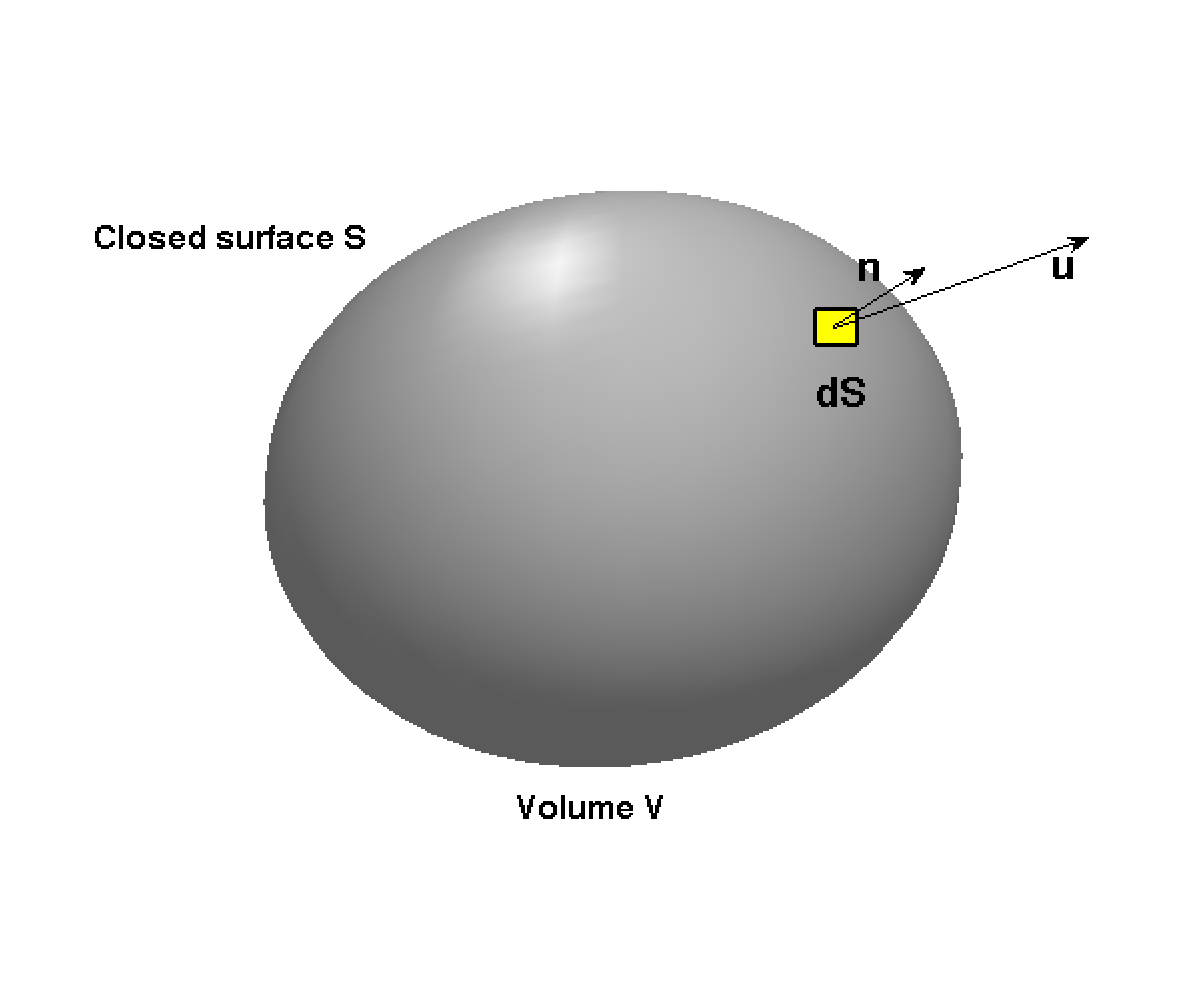
\includegraphics[width=0.5\columnwidth]{\dir/figs/ControlVolume.eps}
  \end{center}
  \caption{Diagram of control volume and associated quantities.}
  \label{fig:controlvol}
\end{figure} 

The value of $\phi$ within $V$ may change over time if:

\begin{enumerate}
\itemsep1pt\parskip0pt\parsep0pt
\item
  There is a flux of $\phi$ through $S$. The flux is partitioned into two parts,
  one due to \href{http://en.wikipedia.org/wiki/Diffusion}{diffusion} and another 
  due to \href{http://en.wikipedia.org/wiki/Advection}{advection}.
\item
  $\phi$ is created or destroyed within $V$.
\end{enumerate}

Formally, the time rate of change in $\phi$ within $V$ is written:

\begin{equation}
{\frac{ \partial }{ \partial t}} { \int }_{ V} \phi dV~ = ~ -{ \int }_{ S} {\mathbf F}
    {\cdot} \hat n~ dS~ - ~{ \int }_{ S} \phi {\mathbf u} {\cdot} \hat n ~ dS~
    + ~{ \int }_{ V} R dV
    \label{eq:intcons}
\end{equation}

where ${\mathbf F}$ represents the flux due to diffusion
($\mathbf{F} \propto \nabla \phi$), $\phi {\mathbf u}$ represents a velocity field 
\emph{advecting} $\phi$, and $R$ represents a source (or sink) of $\phi$. Vector quantities are
represented in \textbf{boldface}. The negative signs in front of the first two terms on the right-hand 
side indicate that an outward flux results in a decrease in $\phi$ within the volume enclosed by $S$.

This statement of conservation of $\phi$ in the unit volume $V$ is always true, independent of the 
size of $V$ and even if the fields enclosed by $S$ are not continuous (this is the case because we
integrate over $V$). It is important to note that that any information on spatial scales smaller than $V$ 
is lost in the process of integration.

% ========================================
\subsection{Derivative form}

Numerical models are often easier to formulate from the derivative form of the conservation equation, and this
is more often the form in which conservation equations are written. This requires the derivatives of $\phi$ to exist 
within $V$, which in turn allows the integral form of the conservation equation to be written as partial differential 
equations, which are upheld within the control volume.

Begin with the terms describing diffusive and advective fluxes into or out of the control volume. The
\href{http://en.wikipedia.org/wiki/Divergence_theorem}{divergence theorem} states that

\begin{equation}
{ \int }_{S} {\mathbf F} {\cdot} \hat{n} ~dS~ = ~{ \int }_{V} \nabla 
    {\cdot} {\mathbf F} ~dV. 
    \label{eq:intcons2}
\end{equation}

Here and below, we will often alternate between standard vector notation (as above) \href{http://en.wikipedia.org/wiki/Index_notation}{and 
indicial (or index) notation}, where a single subscript indicates a component of a vector, two different subscripts indicate a tensor quantity, 
and two repeated subscripts indicate summation. Thus, an identical way of writing equation \eqref{eq:intcons2} is 

\begin{equation}
{ \int }_{ S} {\mathbf F}_{ j} ~n_{ j} ~dS~ = ~{ \int }_{ V} {\frac{
    \partial {\mathbf F}_{ j} }{ \partial x_{ j} }} ~dV.
\end{equation}

Using the divergence theorem, the surface integrals over fluxes in \eqref{eq:intcons} may be replaced by,

\begin{equation}
-{ \int }_{ S} {\mathbf F} {\cdot} \hat{n}dS~ - ~{ \int }_{ S} \phi {\mathbf u}
    {\cdot}\hat{n} dS~ = ~ -{ \int }_{ V} \nabla {\cdot} \left ( {
    {\mathbf F}~ + ~ \phi ~ {\mathbf u}} \right )dV.
\end{equation}

Assuming that the coordinate system is stationary with respect to the velocity field $\mathbf{u}$ 
(i.e, assuming an Eularian reference frame), it is then possible to write

\begin{equation}
{\frac{ \partial}{ \partial t}} { \int }_{ V} \phi ~dV~ = ~{ \int }_{ V}
    {\frac{ \partial \phi }{ \partial t}} ~dV~
\end{equation}

The end result is that the integral form of the conservation equation can now be written as

\begin{equation}
{ \int }_{ V} \left\{ {{\frac{ \partial \phi }{ \partial t}}
    ~ + ~ \nabla {\cdot} \left ( { {\mathbf F}~ + ~ \phi {\mathbf u}} \right ) ~
    - ~ R} \right\} dV~ = ~ 0
\end{equation}

Because $V$ is an arbitrary volume, this equation can only be true if the term in brackets is zero 
for the volume. Hence, for any volume having continuously differentiable $\phi$,

\begin{equation}
{\frac{ \partial \phi }{ \partial t}} ~ + ~ \nabla {\cdot} 
    \left ( { {\mathbf F}~ + ~ \phi {\mathbf u}} \right ) ~ - ~R~ = ~ 0.
    \label{eq:derivcons}
\end{equation}

This is the general form for all conservation laws in continuum mechanics. Below, we apply this to the three quantities conserved in an 
ice sheet (and ideally, in an ice sheet model); mass, energy, and momentum.

% ========================================
\section{Applications of the General Conservation Equation}

%The generalized conservation law in \eqref{eq:derivcons} is now applied to the three quantities conserved in an ice sheet (and
%ideally, in an ice sheet model); mass, energy, and momentum.

% ========================================
% ========================================
\section{Conservation of Momentum}

Starting from Newton's second law of motion, conservation of momentum is expressed as

\begin{equation}
\frac{d} {dt} \int_{V}\rho u_{i}~dV ~ = ~ \int_{V} \frac{\partial \sigma_{ij}} {\partial x_{j}} ~dV +  \int_{V} \rho g_{i}~dV
\label{eq:mobal1}
\end{equation}

where $t$ represents time, $\rho$ represents density, $u$ represents
velocity, $\sigma_{ij}$ represents the stress tensor, $g$ represents the
acceleration due to gravity, $V$ represents the volume of an arbitrary
fluid element, and $(i,j)= \{x, y, z\}$ in a cartesian coordinate
system. Equation \eqref{eq:mobal1} tells us that a fluid element of arbitrary size 
experiences a ``body force'' $\rho g_{i}\delta V$ due to gravity, which is balanced by 
stress divergence $\frac{\partial \sigma_{ij}} {\partial x_{j}} \delta V$ and acceleration
of the fluid in the volume $\delta V$. 

Making the assumptions that we have continuous fields and that ice is incompressible (that is, 
its density $\rho$ does not change under conditions of interest to us), we can write

\begin{equation}
\rho \frac{D u_{i}}{D t}~=~\frac{\partial \sigma_{ij}}{\partial x_{j}} + \rho g_{i}
\label{eq:mobal2}
\end{equation}

in which $D$ is a material derivative. Due to the fact that the \href{http://en.wikipedia.org/wiki/Froude_number}
{Froude number} for ice flow is extremely small, the acceleration term (the first term on the left-hand side) can be 
neglected, leaving the steady-state form, 

\begin{equation}
\frac{\partial \sigma_{ij}}{\partial x_{j}} + \rho g_{i} ~=~0.
\label{eq:mobal3}
\end{equation}

Equation \eqref{eq:mobal3} states that the body force (the gravitational driving force) is balanced by forces resulting from 
gradients in the stress tensor $\sigma_{ij}$. All models of ice-flow dynamics are based on ``solving" this equation in some form.
Chapters \ref{ch:glide} and \ref{ch:glissade} provide additional details on the approximations to this equation that are currently 
solved by Glimmer-CISM.

The \href{http://en.wikipedia.org/wiki/Stress_tensor}{stress tensor} $\sigma_{ij}$ has nine components in our three-dimensional,
cartesian coordinate system,

\begin{equation}
\mathbf{\sigma} =
\left\vert  \begin{array}{ccc} 
    \sigma _{ xx} & \sigma _{ xy} & \sigma _{ xz} \\
    \sigma _{ yx} & \sigma _{ yy} & \sigma _{ yz} \\
    \sigma _{ zx} & \sigma _{ zy} & \sigma _{ zz}. \\
\end{array} \right\vert 
\label{eq:mobal4}
\end{equation}

The components along the diagonal are called normal stresses and the off-diagonal components are called shear stresses. Deformation results
not from the full stress but from the deviatoric stress,

\begin{equation}
\tau_{ ij} ~ = ~ \sigma _{ ij} ~ - ~{\frac{ 1}{ 3}} \sigma _{ kk} \delta _{ ij},
\label{eq:mobal5}
\end{equation}

in which $\delta_{ ij}$ is the Kroneker delta (or the identify tensor). Note that \eqref{eq:mobal5} indicates that for shear stresses, the full
and deviatoric stresses are identical.

\subsubsection{Constitutive relationship}

To relate the stress tensor to fluid motion, we need to introduce the strain rate tensor,

\begin{equation}
\dot{\epsilon}_{ij}~= \frac{1}{2}\left( \frac{ \partial u_{i}}{\partial x_{j}} + \frac{ \partial u_{j}}{\partial x_{i}}\right), ~~i,j = x,y,z,
\label{eq:mobal6}
\end{equation}

where $u_i$ are the velocity vector components. The strain rate tensor $\dot{\epsilon}_{ij}$, and hence gradients in the 
velocity field, is related to the stress tensor $\tau_{ij}$ by a \href{http://en.wikipedia.org/wiki/Constitutive_equation}
{constitutive relation}. For a Newtonian fluid, this can be expressed as,

\begin{equation}
\tau_{ij}~=\eta \dot{\epsilon}_{ij},
\label{eq:mobal7}
\end{equation}

which states that the strain rate is proportional to the stress, with the ice viscosity, $\eta$ serving as the constant of proportionality.
Ice does not behave as a Newtonian fluid, and instead exhibits a \href{http://en.wikipedia.org/wiki/Power-law_fluid}{power-law rheology}, 
so that it becomes more fluid (less viscous) the more it deforms. This relationship can be expressed through Nye's generalization of Glen's 
flow law, 

\begin{equation}
\tau_{ij}~=~A(T^{*})^{\frac{-1}{n}} \dot{\epsilon}_{e}^{\frac{1-n}{n}} \dot{\epsilon}_{ij} 
\label{eq:mobal8}
\end{equation}

in which $T^{*}$ is the absolute temperature corrected for the pressure dependence of the melt temperature, $\dot{\epsilon}_{e}$ is the 
second invariant (a norm) of the stress tensor, and the power-law exponent, $n$, is commonly take as 3. A comparison of Equations 
\eqref{eq:mobal7} and \eqref{eq:mobal8} indicates that one can define an ``effective" ice viscosity for Equation \eqref{eq:mobal7} as

\begin{equation}
\eta_{e}~=~A(T^{*})^{\frac{-1}{n}} \dot{\epsilon}_{e}^{\frac{1-n}{n}}.
\label{eq:mobal9}
\end{equation}

The temperature-dependent rate factor $A$ follows the Arrhenius relationship

\begin{equation}
A\left( T^{*}\right)~=~E A_{o}e^{-Q/RT^{*}},
\label{eq:mobal10}
\end{equation}

in which $A_{o}$ is a constant, $Q$ represents the activation energy for crystal creep, $R$ is the gas constant, and $E$ is a tuning 
parameter, which can be used to account for the effects of impurities and anisotropic ice fabrics. The homologous temperature is

\begin{equation}
T^{*}=T+\rho g H \Phi,
\label{eq:mobal11}
\end{equation}

in which $\Phi$ is 9.8 $\times$10$^{-8}$ K Pa$^{-1}$, or about 8.7 $\times$10$^{-4}$ K m$^{-1}$ in ice. The pressure-dependent melt 
temperature is simply the triple point temperature less the product $\rho g H \Phi$.


% ========================================
% ========================================
\section{Conservation of Energy}
\textbf{SP: This section contains kind of a sloppy interleaving of vector and indicial notation, often within the same
equations. Perhaps we should pick one or the other and stick with it?}

The first law of thermodynamics is used to make a basic statement of conservation of energy in a volume of ice $V$ enclosed within a surface $S$ is

\begin{equation}
\frac{d}{d t} \int_{V}E ~dV~=~- \int_{S}\mathbf{F}\cdot \hat{n}~dS~-~\int_{S}E \mathbf{u}\cdot \hat{n}~dS~+~\int_{V}W dV
\label{eq:enbal1}
\end{equation}

in which $E$ represents the energy of the volume, $F_{i}$ is the flux due
to diffusion, and $W$ represents any sources or sinks of energy within
the volume. The term $Eu_{i}$ is an energy flux through $S$ due to advection.
Following the steps laid out earlier, we use the divergence theorem and
the assumptions of continuous fields and incompressibility, such that

\begin{equation}
\frac{dE}{dt}~+~\nabla \cdot \left(F_{i} +E u_{i}  \right)~-~W~=~0
\label{eq:enbal2}
\end{equation}

Our goal is to use the first law of thermodynamics to compute the temperature of the ice and any changes in that temperature over time.

The energy $E$ is the product of density and the specific internal
energy of the ice $e$, which is itself the product of the specific heat
capacity $c_{p}$ and temperature $T$ (because there is no transfer
between internal energy and pressure for an incompressible fluid). Thus,

\begin{equation}
\begin{matrix}
\frac{dE}{dt}&=&\frac{d\left(\rho e \right)}{dt} \\
&=&\rho\frac{de}{dt}~+~e \frac{d\rho}{dt}\\
&=&\rho c_{p} \frac{dT}{dt}
\end{matrix}
\label{eq:enbal3}
\end{equation}

The heat flux due to diffusion follows Fourier's ``law'' for heat conduction,

\begin{equation}
\begin{matrix}
\nabla \cdot F_{i}&=&\nabla \cdot \left( -k ~\nabla T  \right) \\
&=&-k~\nabla^{2}T,
\end{matrix}
\label{eq:enbal4}
\end{equation}

in which $k$ represents the thermal conductivity of ice and we assume
gradients in its magnitude to be negligible. 
\textbf{SP: Is this true? I thought that one usually kept k (and rho and cp) inside of the 2nd deriv., rather than pulling it out. Maybe Bill can answer this as I am not that familiar with Glimmers heat balance code.}

Using progress made above we can write the advection term

\begin{equation}
\begin{matrix}
\nabla \cdot \left(E u_{i} \right)~=~\rho c_{p}~ u_{i} \cdot \nabla T. 
\end{matrix}
\label{eq:enbal5}
\end{equation}

In the expansion of the terms on the left-hand side of Equation \eqref{eq:enbal5} (using the product rule) we 
have implicitly ignored the term involving $\nabla \cdot u_{i}$ because it is small with respect to the other terms
retained on the right-hand side.

Two quantities must be considered as energy sources, the work done on
the system by internal deformation and the latent heat associated with
phase changes. The former is the product of strain rate and the
deviatoric stress $\dot{\epsilon}_{ij} \tau_{ij}$. The latter is the
product of the latent heat of fusion and the amount of material (ice) subject
to melting (or freezing) per unit volume, per unit time, $L_{f}M_{f}$.

At last, we are able to write equation \eqref{eq:enbal2} in terms of temperature,

\begin{equation}
\frac{\partial T}{\partial t}~=~\frac{k}{\rho c_{p}} \nabla^{2}T~-~u_{i}\cdot \nabla T~+~\frac{1}{\rho c_{p}} \dot{\epsilon}_{ij} \tau_{ij} ~+~\frac{1}{\rho c_{p}} L_{f} M_{f}.
\label{eq:enbal6}
\end{equation}

It is often the case that horizontal terms
$\frac{\partial^{2} T}{\partial x^{2}}$ and
$\frac{\partial^{2} T}{\partial y^{2}}$ are small enough to be ignored.


% ========================================
% ========================================
\subsection{Conservation of Mass}

In this case, $\phi$ from our general conservation equation represents the mass $M$, or more conveniently
$M = \int_V \rho dV$, the integral of the density over the volume. Assuming that there are no sources or 
sinks of mass in the volume ($H$=0), the mass conservation equation is written

\begin{equation}
\int_{V}\frac{\partial \rho} {\partial t} ~dV ~+~ \int_{V} \nabla \cdot \rho \mathbf{u} dV~=~0
\label{eq:mascon1}
\end{equation}

Ice is incompressible (the density does not change in time), which provides the equation for 
local mass continuity,

\begin{equation}
\nabla \cdot \mathbf{u} ~=~0.
\label{eq:mascon2}
\end{equation}

Equation \eqref{eq:mascon2} says that the velocity field is ``divergence free". Applying the $\nabla$ 
operator in cartesian coordinates gives

\begin{equation}
\frac{\partial u_{x}}{\partial x}~+~\frac{\partial u_{y}}{\partial y} ~+\frac{\partial u_{z}}{\partial z}~=~0.  
\label{eq:mascon3}
\end{equation}

To make use of this statement, we need to integrate from the base $b$ to the upper surface $s$ of the ice mass,

\begin{equation}
\int_{b}^{s} \left( \frac{\partial u_{x}}{\partial x}~+~\frac{\partial u_{y}}{\partial y} ~+\frac{\partial u_{z}}{\partial z}\right) dz~=~0.  
\label{eq:mascon4}
\end{equation}

The integral of $\frac{\partial u_z}{\partial z}$ is simply the difference between
the vertical component of the velocity at the upper and lower surfaces, so

\begin{equation}
u_{z} \left(s\right)-u_{z} \left(b\right)~=~-\int_{b}^{s} \frac{\partial u_{x}}{\partial x} dz ~-~\int_{b}^{s} \frac{\partial u_{y}}{\partial y} dz  
\label{eq:mascon5}
\end{equation}

Changing the order of integration and differentiation using the Leibnitz rule we obtain

\begin{equation}
\begin{matrix}
u_{z} \left(s\right)-u_{z} \left(b\right) & = & -~\frac{\partial}{\partial x} \int_{b}^{s} u_{x} dz ~ +~u_{x}(s)\frac{\partial s}{\partial x} ~-~ u_{x}(b)\frac{\partial b}{\partial x}  \\ 
& & -~\frac{\partial}{\partial y}\int_{b}^{s} u_{y} dz   ~ +~u_{y}(s)\frac{\partial s}{\partial y} ~-~ u_{y}(b)\frac{\partial b}{\partial x}.
\end{matrix}
\label{eq:mascon6}
\end{equation}

The vertical velocity at the upper surface $u_{z}(s)$ is the result of motion parallel to the surface slope, 
the rate of new ice accumulation $\dot{a}$, and any time-change in the surface height,

\begin{equation}
u_{z} \left(s\right)~=~\frac{\partial s}{\partial t}~+~u_{x}(s)\frac{\partial s}{\partial x}~+~u_{y}(s)\frac{\partial s}{\partial y}~-~\dot{a}, 
\label{eq:mascon7}
\end{equation}

recognizing that a negative accumulation rate indicates ablation. Similarly, the vertical velocity at the lower surface is

\begin{equation}
u_{z} \left(b\right)~=~\frac{\partial b}{\partial t}~+~u_{x}(b)\frac{\partial b}{\partial x}~+~u_{y}(b)\frac{\partial b}{\partial y}~-~\dot{b} 
\label{eq:mascon8}
\end{equation}

in which $\dot{b}$ represents the basal accumulation rate.

Substituting equations \eqref{eq:mascon7} and \eqref{eq:mascon8} into \eqref{eq:mascon6} we find that many terms cancel,

\begin{equation}
\frac{\partial s}{\partial t}~-~\dot{a}~-~\frac{\partial b}{\partial t}~+~\dot{b}~=~-~\frac{\partial}{\partial x} \int_{b}^{s} u_{x} dz~-~\frac{\partial}{\partial y} \int_{b}^{s} u_{y} dz.
\label{eq:mascon9}
\end{equation}

Finally, making the substitution that the ice thickness $h=s-b$ we obtain

\begin{equation}
\frac{\partial h}{\partial t}~=~-~\frac{\partial}{\partial x} \int_{b}^{s} u_{x} dz~-~\frac{\partial}{\partial y} \int_{b}^{s} u_{y} dz ~+~\dot{a}~-~\dot{b}.
\label{eq:mascon10}
\end{equation}

If we integrate in the vertical, we get 

\begin{equation}
\frac{\partial h}{\partial t}~=~-~\nabla \cdot \left( U_{i} h \right) +~\dot{a}~-~\dot{b}
\label{eq:mascon11}
\end{equation}

in which $U_{i}$ represents the vertically averaged velocity, i.e. $U_i = \frac{1}{h}\int_{b}^{s}u_{i}dz$ . Note that this equation is 
prognostic; we can use the current velocity and geometry of the ice to compute a rate of change in the geometry.


% ========================================
% ========================================

%\section{Numerical Solutions of the Field Equations}

%3D, thermo-mechanically coupled ice sheet models. 3D refers to the
%explicit vertical layering of the model for computing temperature.
%Thermo-mechanical means that the ice viscosity is sensitive to
%temperature, and an iterative procedure must be used to find the flow
%rates from temperature. Both models exploit the often used shallow ice
%approximation \textbackslash{}citep\{hutter83\}, which accounts for the
%membrane like nature of ice sheets by reducing the stress tensor to only
%leading order terms resulting from simple shear. The shallow ice
%approximation, when combined with the non-linear constituative relation
%given by Glen's flow law \textbackslash{}citep\{paterson94\}, leads to
%the following expression for horizontal velocities
%
%$\begin{matrix}
%u_i(z) &=& -2 (\rho g)^n \vert \nabla s\vert ^{n-1} \frac{\partial s}{\partial i} 
%\int_h^z A(\theta^*)(s-z)^n dz + u_i(h)\\
%i &=& x,y.
%\end{matrix}$
%
%All parameters and symbols used in this paper appear in table
%\textbackslash{}ref\{symbols\}. It is worth noting that all quantities
%used to find the horizontal velocities are computed locally. The shallow
%ice approximation eliminates terms resulting from transverse or lateral
%stresses. The temperature sensitivity of ice flow is given by an
%Arrhenius relation,
%
%$
%A(\theta^*) = a \exp \left(\frac{-Q}{R\theta^*}\right).
%$
%
%Which, in typical ice temperature ranges (-50 -{}- 0 C$^\circ$) varies
%over 3 orders of magnitude. However because most shear occurs at the
%base, and the base is warmed by dissipation and geothermal heat flow, a
%more appropriate range is -20 -{}- 0 C$^\circ$. This gives a range of
%$A$ over about a factor of 30.
%
%Assuming that horizontal diffusion is negligible, again due to the
%membrane nature or very small aspect ratio (ratio of vertical to lateral
%extent) of ice sheets, the ice temperature field is found from the
%conservation of energy
%
%$ 
%\frac{\partial \theta}{\partial t} = \frac{k}{\rho c}
%\frac{\partial^2
%\theta}{\partial z^2} -
%\mathbf{u} \cdot \nabla \theta -
%u_z \frac{\partial \theta}{\partial z} 
%+ \frac{g(s-z)}{c}\frac{\partial \mathbf{u}}{\partial z} \cdot \nabla s.
%$
%
%The terms on the right hand side from left to right are vertical
%diffusion, horizontal advection, vertical advection, and dissipation
%(using only the shallow ice stress tensor). Equation
%\textbackslash{}ref\{temp\} is subject to the boundary conditions
%
%$\begin{matrix}
%\theta - \theta_s(x,y) = & 0 &~\forall z=s \\
%k \nabla \theta \cdot \mathbf{\hat n}(h) =& -G(x,y) + \mathbf{u} \cdot \tau_d
%&~\forall z=h.
%\end{matrix}$
%
%The upper surface is set to a mean annual temperature ($\theta_s$), and
%the lower surface is accounting for the heat sources from both
%geothermal heat ($G$) flux, and frictional heat generated when ice
%slides over the bed. The temperatures are constrained by the melting
%point corrected for pressure via the Clausius-{}-Clapeyron gradient
%
%$
%\theta^* = \theta - \beta (s-z)
%$
%
%The vertical advection term in equation \textbackslash{}ref\{temp\}
%requires vertical velocities. They are found from incompressibility,
%
%$
%\frac{\partial u_x}{\partial x} + 
%\frac{\partial u_y}{\partial y} +
%\frac{\partial u_z}{\partial z} = 0,
%$
%
%by integrating with respect to $z$, giving
%
%$
%u_z(z) = -\int_h^z \left( \frac{\partial u_x}{\partial x} + \frac{\partial
%u_y}{\partial y}\right ) dz + M + \mathbf{u}(h) \cdot \nabla h.
%$
%
%Were the complete accounting must include the melt rate and bed
%topography. Basal melt rates computed from the jump boundary condition
%at the bed,
%
%$
%M = \frac{1}{\rho L} \left ( k \frac{\partial
%\theta(h)}{\partial z} + G + \mathbf{u} \cdot \tau_d \right ).
%$
%
%Having solved for the temperature dependent velocity fields, changes in
%the ice sheet's geometry are computed from the continuity equation
%
%$
%\frac{\partial H}{\partial t} = - \nabla \cdot (\mathbf{\bar u} H) + B - M.
%$
%
%Both models use the finite difference methods for descritization of the
%partial differential equations. GLIMMER differs from PISM in that it
%offers a choice of implicit schemes for solving equation
%\textbackslash{}ref\{continuity\}, whereas PISM uses an explicit scheme
%\textbackslash{}citep\{press92\}. Further, GLIMMER utilizes a rescaled,
%or $\sigma$ vertical coordinate \textbackslash{}citep\{lliboutry87\} and
%PISM does not. PISM uses the PETSc
%\textbackslash{}citep\{petsc-user-ref\} library to achieve parallelism
%and has the capacity to include a more complete stress formulation, but
%that capacity was not used here. Additional discussion of the field
%equations and numerical methods used in GLIMMER can be found in
%\textbackslash{}citet\{payne97\} and \textbackslash{}citet\{payne99\}.
%
%The ice sheet model CISM uses a finite difference method to solve the
%governing thermodynamic equations for ice using the \{\textbackslash{}it
%shallow ice approximation\}. This is the approach generally adopted for
%modeling large ice masses. The assumption is made that slopes at the
%upper and lower surfaces are sufficiently small that normal stress
%components can be neglected. This leads to a \{\textbackslash{}it
%local\} balance between the gravitational driving stress and the basal
%shear stress and expressions for the shear stresses
%
%$\begin{matrix}
%\tau_{xz}(z)&=&-\rho g \left(s - z \right) \frac{\partial s}{\partial x}  \\
%\tau_{yz}(z)&=&-\rho g \left(s - z \right) \frac{\partial s}{\partial y}
%\end{matrix}$
%
%Evolution of the ice thickness uses equation
%\textbackslash{}ref\{equation:mabalfinc\} and the temperature solver
%uses a version of equation \textbackslash{}ref\{equation:enbalfin\}
%simplified to neglect horizontal diffusion (a typical simplification).
%
%The model equations are solved on a regular grid using the Glen flow law
%(equation \textbackslash{}ref\{equation:Glen\}) and appropriate boundary
%conditions for the upper and lower surfaces. These include the surface
%ice accumulation rate and temperature and a geothermal gradient (applied
%at the base of a bedrock layer with specified thermal properties). Basal
%traction may also be specified, in the situation where ice is at the
%melt temperature at the base. Isostatic adjustment of the land surface
%beneath the ice sheet, not discussed here, is also included.
%
%\subsubsection{numerical scheme}
%
%The continuous functions represented by the model governing equations
%cannot be solved exactly. Instead, they are discretized so that finite
%approximations of their solutions may be made. There are a variety of
%numerical techniques available for this purpose, GLIMMER makes use of a
%finite difference method.
%
%In brief, the model domain (a region of Earth's surface, for example,
%Greenland) is subdivided into a regularly-spaced horizontal grid and
%derivatives are approximated along the grid directions. The grid is
%fixed in space over the course of the model run. Model variables such as
%ice thickness are updated at each time step according to the numerical
%approximations of the governing equations. The vertical dimension is
%treated using a non-dimensional ``stretch'' coordinate so that an
%evolving ice thickness may be accommodated. The scaling is:
%
%$
%\zeta~=~\frac{s-z}{H}
%$
%
%so that $\zeta=1$ at the surface $s$ and $\zeta=0$ at the base. The
%governing equations must be re-written in the new, $(x, y, \zeta)$
%coordinate system.
%
%If you would like to read more about the inner workings of GLIMMER, its
%documentation is available at the class website. This is not necessary
%for the present lab exercise.






% ========================================
